\section{The finite action protocol}
\label{sec:yba-appendix}
\label{app:actions}

For the finite selector, set \(K_u=C_u-\beta G_u\) and
\(r_u=\mu_ue^{-K_u/\tau}/Z\). Substitution gives
\begin{align}
 \Phi(P)
 &=\tau\sum_uP_u\log\frac{P_u}{r_u}-\tau\log Z .
 \label{eq:selector-proof}
\end{align}
Nonnegativity of relative entropy gives the unique minimiser \(r\). Positive \(\mu_u\), finite \(K_u\), a finite action set and \(\tau>0\) ensure full support. Hard exclusions should instead be represented by removing unavailable actions or restricting support explicitly. They are not part of the positive-mass proof.

The deterministic policy used in the tracking calculation compares \(\beta G_u-C_u\) for two equal-reference-mass actions and uses strict inequality to buy an update. Its score is not a statement that an action was sampled. A different tie rule changes a deterministic transition at equality and must be retained with the state protocol.

The actual trailing window is
\(D_t=\{\max(0,t-27),\ldots,t\}\).
For a generic target displacement \(v\), direct expansion of
\((y_i-(\vartheta+\rho v)x_i)^2\) gives Eq.~\eqref{eq:partial-gain}. At the unregularised least-squares target,
\(B_t-A_t\vartheta=A_tv\), so
\(G_{\mathrm{partial}}=(2\rho-\rho^2)A_tv^2\).
The full-fit gain is \(A_tv^2\). A ridge target does not satisfy that first equality exactly.

Finite branch controls used constant observations \(x_i=1,y_i=0.8\), the same partial-step scorer, and the same strict selection/application path. At price \(0.02\), an eight-observation call promotes from 1 to \(0.9559999780000028\). A nine-observation call reusing the actual carried state promotes to \(0.9216799632844488\). At price \(0.06\), the eight-observation call stays. At the positive executable tie price \(0.039160017159996584\), recomputed binary64 scores are exactly equal and the policy stays.

An independent rational oracle uses
\[
 \vartheta_{\mathrm w}=\frac{n(4/5)}{n+1/10^6},\quad
 \vartheta_1=\vartheta+\frac{11}{50}(\vartheta_{\mathrm w}-\vartheta),
\]
and \(G_1=2\delta(4/5-\vartheta)-\delta^2\), with
\(\delta=\vartheta_1-\vartheta\).
The largest recorded state/gain/score residual in the four-case control was \(6.25\times10^{-17}\), below the predeclared \(10^{-12}\) tolerance. An exact floating-point score tie is a branch observation, not an assertion that binary arithmetic equals its rational idealisation.

\section{Proof of weighted classical contraction}
\label{app:classical}

For a positive receiving mass \(q_y\), write
\(p_x=q_yr_y(x)\) on \(\pi^{-1}(y)\). Define
\[
 Z_y=\sum_{\pi(x)=y}w_xe^{-K_x/\tau},
 \qquad r_y^*(x)=\frac{w_xe^{-K_x/\tau}}{Z_y}.
\]
Since \(K_{\mathrm{eff}}(y)=-\tau\log(Z_y/w_y)\),
\begin{align}
 \mathcal J_X(p)
 ={}&\sum_yq_yK_{\mathrm{eff}}(y)
       +\tau\sum_yq_y\log(q_y/w_y)\nonumber\\
    &+\tau\sum_yq_yD(r_y\Vert r_y^*).
 \label{eq:conditional-kl}
\end{align}
Zero-mass fibres contribute zero under \(0\log0=0\). All other conditional relative entropies can be minimised independently. This proves Eq.~\eqref{eq:contraction} without an assumption about how a dynamical learner explores the fibre.

For a further surjection \(\psi:Y\to Z\), let
\(w_z=\sum_{\psi(y)=z}w_y\). Then
\begin{align}
 &\sum_{\psi(y)=z}\frac{w_y}{w_z}e^{-K_{\mathrm{eff}}(y)/\tau}
 \nonumber\\
 &\hspace{1em}=
 \sum_{(\psi\circ\pi)(x)=z}\frac{w_x}{w_z}e^{-K_x/\tau}.
 \label{eq:staged-contraction}
\end{align}
Direct and staged elimination therefore agree. A change in reference convention must be included before comparing generators. Restricted parametrisations and repeated projection back into them are additional operations and need not preserve this associativity.

\section{Convergence of the reuse-mode controller}
\label{app:controller}

Each component of Eq.~\eqref{eq:regulator} is a convex combination of values in \([-1,1]\), so the square is invariant. For two states at a common frozen \(h\), the Lipschitz property of \(\tanh\) gives
\begin{align*}
 |\delta m^+|&\leq(1-a_m)|\delta m|+a_m|\delta\lambda|,\\
 |\delta\lambda^+|/\nu
 &\leq(1-a_\lambda)|\delta\lambda|/\nu
             +(a_\lambda k/\nu)|\delta m|.
\end{align*}
Taking the weighted maximum gives the factor \(r<1\) in Eq.~\eqref{eq:contraction-factor}. The closed square is complete in this norm. The contraction theorem supplies a unique fixed point and the geometric bound
\(\|z_n-z^*\|_\nu\leq r^n\|z_0-z^*\|_\nu\).
An uncontractive continuous self-map of a compact convex state domain may still have a fixed point, but continuity alone does not supply attraction.

The parameter restriction \(k<1\) is sufficient, not a theorem that all larger couplings fail. A switched register or changing \(h\) is a different problem. The retained finite checks corroborate examples of this fixed-drive map, not every parent-learning extension.

Suppose a specified external improvement field in the same model metric is \(g_{\mathrm{ext}}\). Exact alignment
\(-\operatorname{grad}_m J=g_{\mathrm{ext}}\) is an additional premise. At a stationary gradient-model state it implies \(g_{\mathrm{ext}}=0\). With alignment defect at most \(\varepsilon\), stationarity bounds \(\|g_{\mathrm{ext}}\|\) by \(\varepsilon\). A fixed-point equation alone provides neither premise. On a neighbourhood, representing a prescribed field by a scalar loss also requires the relevant integrability conditions.

\section{The OR figure protocol}
\label{app:or-protocol}

Under the declared independent product law, summing binary path weights gives \(Z_B=e^{h_B}\). The empty path weighs 1, so the nonempty probability is \((Z_B-1)/Z_B\). Its log odds are \(\log(e^{h_B}-1)\). Differentiating at fixed margins gives
\[
 \frac{dh_B}{dc}=-\sum_tp_t,\qquad
 \frac{d\,\operatorname{logit}q_B}{dc}
                  =-\frac{\sum_tp_t}{q_B}.
\]
Because \(N_B=0\) on the empty event,
\(\mathbb E N_B=q_B\mathbb E[N_B\mid N_B\geq1]\).
This proves Eq.~\eqref{eq:multiplicity}. For more than one finite logistic opportunity, both one event and multiple events have positive conditional probability, giving the strict bounds.

The four externally frozen margin blocks in Fig.~\ref{fig:num-toy-coarse-defect} are the rows of
\[
 \begin{pmatrix}
 -0.4&0.2&0.9&-0.1\\
 0.1&0.1&0.1&0.1\\
 0.7&-0.5&0.7&-0.5\\
 -0.2&-0.2&0.2&0.2
 \end{pmatrix}.
\]
The 81 equally spaced prices run from \(0.001\) to 2 inclusive. At each price, the naive law uses \(\sigma(S_B-c)\). The restricted fitted law uses the arithmetic mean of the four exact block intercepts. Mean TV averages the four absolute event-probability errors. Maximum TV takes their maximum. Multiplicity curves give the mean, minimum and maximum of \(\sum_tp_t/q_B\) over blocks.

The numerical implementation uses stable softplus and exponential expressions in double precision. The maximum recorded difference between exact hazard and the OR product was \(2.220446049250313\times10^{-16}\). This is numerical agreement with an algebraic identity. It is not an observed instability threshold or a fit to the adaptive tracking process.

The full function \(h_B(c)\), rather than one number \(h_B(c_0)\), is available for repricing because the margin schedules are retained. Replacing every block by the mean intercept is a projection. Repeating that projection after regrouping blocks need not reproduce direct elimination, even though exact hazard merging is associative.

\section{Bounds for receiving dynamics}
\label{app:maps}

For a differentiable receiving map \(\pi\), write \(x(t)\) for the fine trajectory and \(y(t)\) for the proposed receiving trajectory, with \(y(0)=\pi x(0)\). Suppose both remain in a declared receiving domain for \(0\leq t\leq T\), that \(w\) is \(L\)-Lipschitz there, and that
\(\|D\pi_xv(x)-w(\pi x)\|\leq\delta_0\) along the relevant fine paths. Adding and subtracting \(w(\pi x(t))\) gives
\[
 \|\pi x(t)-y(t)\|
 \leq\int_0^t[\delta_0+L\|\pi x(s)-y(s)\|]\,ds .
\]
Gronwall's inequality yields
\[
 \|\pi x(t)-y(t)\|\leq
 \begin{cases}
 \delta_0(e^{Lt}-1)/L,&L>0,\\
 \delta_0t,&L=0 .
 \end{cases}
\]
The metric cannot be changed midway through the comparison. For invertible coordinate maps, consistent field transport makes the local mismatch vanish. A coarse map need not admit any autonomous field \(w\) with zero mismatch.

For finite kernels, let \(\mu_n\) be the fine law and \(\nu_n\) the proposed receiving law, with \(\nu_0=\pi_*\mu_0\). The uniform defect in Eq.~\eqref{eq:kernel-defect} implies
\[
 \|\pi_*(\mu_nP)-(\pi_*\mu_n)Q\|_{\mathrm{TV}}\leq\epsilon .
\]
Adding and subtracting \((\pi_*\mu_n)Q\), then using TV contraction under \(Q\), gives
\(d_{n+1}\leq\epsilon+d_n\).
Consequently \(d_n\leq\min(1,n\epsilon)\). This is a worst-case finite-horizon statement. A smaller averaged defect requires its own state distribution and does not automatically imply the uniform bound.

\section{Logarithmic capacity costs}
\label{app:rank}

A multiplicative capacity coordinate gives a useful special case of the price ledger. Suppose
\(f:\mathbb N\to\mathbb R_{\geq0}\) is nondecreasing and obeys
\(f(rs)=f(r)+f(s)\).
Then \(f(1)=0\). If \(f(2)=0\), bounding any \(n\) by a power of two forces \(f(n)=0\). Otherwise put \(k_j=\lfloor j\log_2n\rfloor\). Monotonicity gives
\[
 k_jf(2)\leq jf(n)\leq(k_j+1)f(2).
\]
Dividing by \(j\) and taking the limit proves
\(f(n)=\kappa\log n\), with \(\kappa=f(2)/\log2\geq0\).
The composition premise concerns a declared capacity label. It is not implied by statistical independence of probability-order ranks.

For example, marginal probabilities \((0.7,0.3)\) and \((0.6,0.4)\) produce joint probabilities \(0.42,0.28,0.18,0.12\). The pair with marginal ranks \(2,1\) has joint probability-order rank 3, not their product 2. If labels are instead explicitly multiplicative capacities, their multiplicities remain in the reference measure. Write \(I>0\) for the inverse statistical cost scale when the cost is \(\log r\). Two factors labelled \(\{1,2\}\) produce \(\{1,2,2,4\}\), so their cost-weighted partition sum is \((1+2^{-I})^2\).

A separate consecutive-label model has one alternative at each \(r=1,\ldots,R\). With equal reference masses, equal gains, cost \(\log r\) and inverse cost scale \(I\), the selector specialises to
\[
 p_I(r)=\frac{r^{-I}}{Z_R(I)},\qquad
 Z_R(I)=\sum_{r=1}^Rr^{-I}.
\]
This follows from the stated maximum-entropy or relative-entropy selection premise, not from a universal empirical rank law. Its response satisfies
\[
 -\partial_I\log Z_R=\mathbb E_I\log r,\qquad
 \partial_I^2\log Z_R=\operatorname{Var}_I(\log r).
\]
The infinite consecutive-label limit is normalised by \(\zeta(I)\) only for \(I>1\). Finite representational systems keep their actual cutoff and multiplicities.
\section{A finite comparison of priced update policies}
\label{app:protocol}

Twelve predeclared streams, seeds \(0,\ldots,11\), each contain 700 observations indexed \(0,\ldots,699\). Inputs are independent standard normal draws and \(y_t=\vartheta_t^*x_t+\xi_t\), with independent Gaussian noise of standard deviation \(0.25\). The true slope starts at 1 and becomes \(1.75,0.6,1.45,1.05\) at observations \(140,310,470,600\). Each seed's observations are reused for all three policies and prices \(c\in\{0.001,0.005,0.02,0.06,0.12,0.4\}\). States start at 1. The 216 trajectories comprise 150984 decisions. Parameters are \(\beta=2.5\), window length 28, minimum eight fit points, ridge denominator \(10^{-6}\), partial step \(0.22\). No price is selected as an optimum.

We define the three mechanisms once. The \emph{full-fit-scored noisy-step policy} scores \(G_{\rm full}=\max(0,J_t(\vartheta)-J_t(\vartheta_{\mathrm w}))\) against proxy \(g_0=0.1\min((y_t-\vartheta x_t)^2,0.25^2)\), but applies a partial step towards \(\operatorname{clip}(y_t/x_t,-1.5,3.5)\), falling back to the rolling fit when \(|x_t|\leq0.15\). The \emph{full-fit-scored rolling control} uses that full-fit/proxy scoring but applies the partial rolling-fit action of Eq.~\eqref{eq:actions}. The \emph{actual-step-priced rolling policy} scores that actual candidate directly and gives staying zero gain. Each buys an update iff its declared \(\beta(G_1-G_0)>c\), pays \(c\), and otherwise carries the unchanged state. The first two policies' positive proxy is not a realised no-update improvement. The rolling control isolates action-target change from the combined repricing of the partial step and staying baseline.

Prediction uses the state available \emph{before} the current observation updates it. Mean squared prediction error and promotion fractions use \(t=50,\ldots,699\), hence 650 observations per stream. Charged cost per evaluated observation is \(c\) times promotion fraction. It excludes controller computation and maintenance and is not measured energy. A fixed-slope-1 baseline and privileged true-slope predictor have mean errors \(0.2899961\) and \(0.0628541\). Truth is used only for evaluation. Table~\ref{tab:policies} retains all six matched prices. Actual-step pricing has higher mean error than the noisy-step policy throughout. At \(c=0.06\), it also has essentially the same, slightly higher charged cost. At some other prices it buys fewer updates while predicting worse. Internal gain accounting supplies no dominance conclusion.

\begin{table*}[t]
\centering
\caption{Matched synthetic comparison. N, R and A denote the full-fit-scored noisy-step policy, full-fit-scored rolling control and actual-step-priced rolling policy defined in Appendix~\ref{app:protocol}. Entries average 12 streams. Promotion fraction is updates/650. Failure averages each stream's four-shift fraction without a qualifying in-band run. These are descriptive means, not an optimum or independent-shift uncertainty estimate.}
\label{tab:policies}
\begin{tabular}{c|ccc|ccc|ccc}
\hline
&\multicolumn{3}{c|}{Prediction MSE}&\multicolumn{3}{c|}{Promotion fraction}&\multicolumn{3}{c}{Unrecovered fraction}\\
\(c\)&N&R&A&N&R&A&N&R&A\\ \hline
0.001&0.105146&0.120979&0.119865&0.307308&0.291026&0.365769&0&0.020833&0\\
0.005&0.104527&0.121233&0.120905&0.198718&0.210385&0.186795&0.020833&0.041667&0.083333\\
0.02&0.111496&0.123236&0.126844&0.100897&0.138718&0.103077&0.020833&0.083333&0.208333\\
0.06&0.121170&0.129231&0.143405&0.050385&0.088590&0.050769&0.187500&0.270833&0.625000\\
0.12&0.131270&0.139036&0.161741&0.035256&0.059359&0.029615&0.291667&0.458333&0.895833\\
0.4&0.170679&0.174570&0.236637&0.018590&0.022564&0.007051&0.937500&0.895833&0.770833\\ \hline
\end{tabular}
\end{table*}

At a true shift \(s\), a qualifying run is five consecutive pre-action estimates within \(20\%\) of the jump magnitude, entirely inside \([s,s+65)\). Delay is the first run's \emph{start}, not confirmation four observations later. Already-in-band estimates qualify without a new promotion. Thus recovery measures target occupancy, not detected change or update-triggered success. Without a qualifying run, the shift fails and sentinel delay 65 remains in the capped-delay mean. Four shifts in 12 streams give 48 dependent evaluations per policy/price. Occupancy need not be monotone in price: a model already near the last target can qualify without reacting successfully to preceding shifts.

An off-transition frequency excludes the four nonoverlapping 65-step post-shift windows, leaving 390 evaluated observations per stream. Its denominator is 390, not the number of promotions, and it is not a false-positive probability. Each mean averages 12 stream-level quantities. Descriptive SE is the sample standard deviation divided by \(\sqrt{12}\). Paired comparisons subtract same-seed errors before computing SE. No binomial uncertainty based on 48 independent shifts is used. Realised gains on overlapping windows cannot be summed into additive forecast improvement.

Reference controls matched six seed-0 noisy-step trajectories to the original policy and three predeclared seed-0 actual-step trajectories to the selection/application implementation, with recorded zero state discrepancy and identical choices under tolerance \(10^{-12}\). Actual-step candidate-versus-realised accounting discrepancy was zero on recorded paths. These controls establish finite implementation agreement, whereas the observations establish the finite predictive comparison. The executed calculations used Python 3.14.7 and NumPy 2.5.1. No new scientific run was made to produce this manuscript.


\subsection{Updates outside post-shift windows}

Figure~\ref{fig:off-transition} asks where revisions are spent outside the post-shift windows. Excluding the four nonoverlapping 65-step post-shift windows from the 650-observation evaluation interval leaves 390 observations per stream. The off-transition rate is purchased updates in those observations divided by 390. It is not the share of promotions that were false, and it is not a false-positive probability. Useful adaptation to noisy observations can occur between the designated latent shifts.

\begin{figure*}[t]
\centering
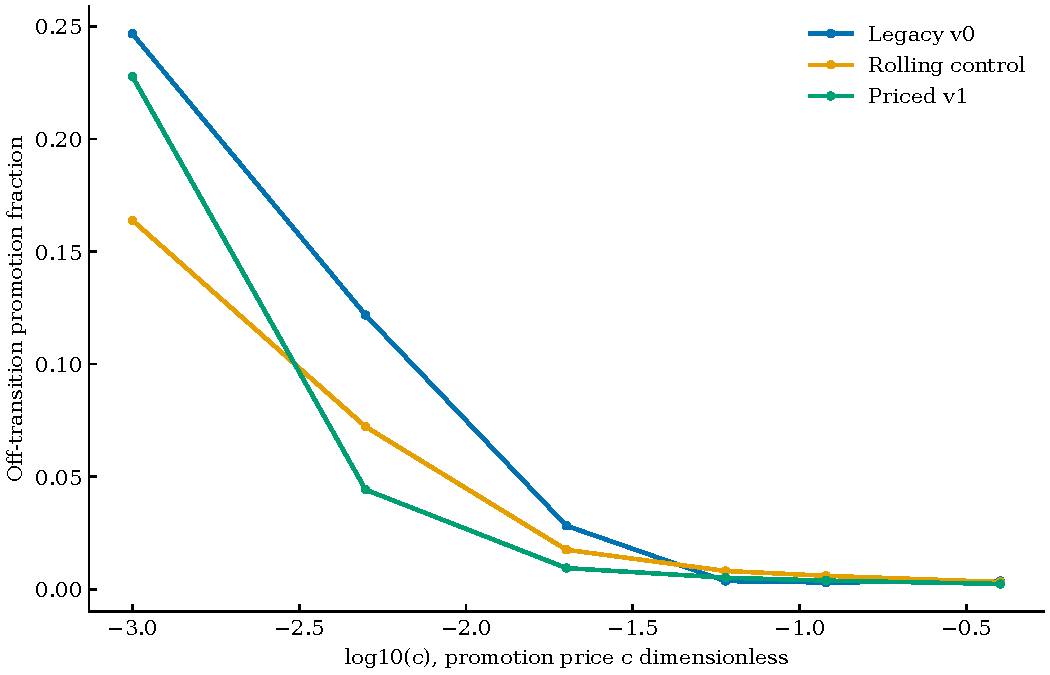
\includegraphics[width=0.84\textwidth]{figures/generated/slg-off-transition-promotions-20261111.pdf}
\caption{Updates outside the declared post-shift windows. Promotion fraction over observations \(50\)--\(699\) excluding each interval \([s,s+65)\) beginning at a true shift \(s\), averaged over 12 matched streams. The denominator is 390 observations per stream, not the number of updates. The same three methods and prices are used as in the main comparison. This operational rate is not a false-positive probability. Read with prediction risk and target occupancy before treating suppressed updates as improved adaptation. Lines show finite stream means without uncertainty bands.}
\label{fig:off-transition}
\label{fig:slg-off-transition-promotions-20261111}
\end{figure*}

\section{Quantum contraction as feasible recovery}
\label{app:quantum}

The classical fibre proof relies on the possibility of choosing conditional distributions independently at a fixed marginal. Quantum constraints require a different equality test. Let a finite Hermitian generator \(K\) act on finite-dimensional \(S\otimes E\). For \(\tau>0\), define
\[
 \omega=\frac{e^{-K/\tau}}{Z},\qquad
 Z=\operatorname{Tr}e^{-K/\tau},\qquad
 \omega_S=\operatorname{Tr}_E\omega .
\]
Both reference states are faithful. With von Neumann entropy
\(S(\rho)=-\operatorname{Tr}\rho\log\rho\), the free-energy functional is
\begin{equation}
 \mathcal J_K(\rho)=\operatorname{Tr}\rho K-\tau S(\rho)
       =\tau D(\rho\Vert\omega)-\tau\log Z .
 \label{eq:quantum-free-energy}
\end{equation}
The equilibrium marginal generator
\[
 K_{\mathrm{eff}}=-\tau\log\operatorname{Tr}_Ee^{-K/\tau}
\]
reproduces \(\omega_S=e^{-K_{\mathrm{eff}}/\tau}/Z\) exactly. This equilibrium identity is distinct from minimising over extensions of an arbitrary prescribed marginal \(\sigma\).

Here \(D(\rho\Vert\omega)=\operatorname{Tr}[\rho(\log\rho-\log\omega)]\) is quantum relative entropy, with \(0\log0=0\). The receiving functional is
\[
 \mathcal J_{\mathrm{eff}}(\sigma)
 =\operatorname{Tr}\sigma K_{\mathrm{eff}}-\tau S(\sigma)
 =\tau D(\sigma\Vert\omega_S)-\tau\log Z .
\]
Define the constrained value by
\begin{align}
 C(\sigma)&=\min_{\rho:\operatorname{Tr}_E\rho=\sigma}
                         \mathcal J_K(\rho)\nonumber\\
 &=\mathcal J_{\mathrm{eff}}(\sigma)+\Delta_Q(\sigma),
 \label{eq:quantum-contraction}
\end{align}
where
\begin{equation}
 \Delta_Q(\sigma)=
 \tau\min_{\rho:\operatorname{Tr}_E\rho=\sigma}
 [D(\rho\Vert\omega)-D(\sigma\Vert\omega_S)]\geq0 .
 \label{eq:quantum-gap}
\end{equation}
The extension set is nonempty and compact. The entropy functional is continuous with \(0\log0=0\), so a minimiser exists even for singular \(\sigma\). Nonnegativity is relative-entropy data processing under partial trace \cite{PETZ200347a4ef,Junge20189e4744}.

For the faithful reference, the fixed-reference Petz map is
\begin{equation}
 \mathcal R_\omega(X)=\omega^{1/2}
 [\omega_S^{-1/2}X\omega_S^{-1/2}\otimes I_E]\omega^{1/2}.
 \label{eq:petz-map}
\end{equation}
It is completely positive and trace preserving and maps \(\omega_S\) to \(\omega\). The equality/recovery theorem, with its support convention \cite{Junge20189e4744}, gives
\begin{equation}
 \Delta_Q(\sigma)=0
 \quad\Longleftrightarrow\quad
 \operatorname{Tr}_E\mathcal R_\omega(\sigma)=\sigma .
 \label{eq:recovery-feasibility}
\end{equation}
Necessity follows because an extension saturating data processing must be recovered by this map. For sufficiency, the displayed marginal condition makes \(\mathcal R_\omega(\sigma)\) feasible. Apply data processing first under partial trace and then under \(\mathcal R_\omega\). Since the reference is returned in both directions, the two inequalities force equality. No inverse of the target \(\sigma\) is used. A nonfaithful reference would require inverses on its support and additional support restrictions, outside this statement.

For a product generator
\(K=K_S\otimes I+I\otimes K_E\),
recovery is \(\sigma\otimes\omega_E\) for every target \(\sigma\). For a classical-quantum block generator
\[
 K=\sum_s|s\rangle\langle s|\otimes K_E(s),
\]
targets diagonal in that retained basis,
\(\sigma=\sum_sq_s|s\rangle\langle s|\), have the feasible optimal extension
\[
 \rho^*=\sum_sq_s|s\rangle\langle s|\otimes
 \frac{e^{-K_E(s)/\tau}}{\operatorname{Tr}e^{-K_E(s)/\tau}} .
\]
These controls specify both the retained algebra and the allowed target states. A diagonal interaction does not allow every coherent target.

For a counterexample, take \(K=gZ_S\otimes Z_E\), with Pauli \(Z\), and \(\sigma=|+x\rangle\langle+x|\). A pure marginal forces every extension to be \(\sigma\otimes\rho_E\). Its interaction expectation is zero, so maximising the environmental entropy gives \(C(\sigma)=-\tau\log2\). Yet
\(K_{\mathrm{eff}}=-\tau\log[2\cosh(g/\tau)]I\), and therefore
\begin{equation}
 \Delta_Q(\sigma)=\tau\log\cosh(g/\tau)>0
                         \quad(g\ne0).
 \label{eq:quantum-witness}
\end{equation}
Even \([\sigma,\omega_S]=0\) holds because \(\omega_S=I/2\). That commutation is not enough to make recovery feasible. The analogous \(X\otimes X\) interaction with a pure \(z\)-target gives the same gap. At \(\sigma=I/2\), the Gibbs extension is feasible and the gap vanishes, so a state-independent correction cannot repair the entire constrained functional.

The retained \(4\times4\) controls at \(\tau=1,g=0.7\) give gap \(0.2272702294\) for both coherent witnesses, agreeing with \(\log\cosh(0.7)\). Product and declared diagonal-target controls have zero gap within the recorded tolerance. These controls evaluate analytically identified minimisers. They are not an unrestricted numerical optimisation over every quantum extension.

\section{Reproducibility}
\label{app:evidence-scope}

The source package retains the exact figure PDF hashes, plotted data tables, source code, environment and finite protocols. The synthetic comparison uses the observations, prices, prediction timing and occupancy rules stated above. The analytic controls, finite action-branch controls and long-horizon policy comparison answer different questions. No new numerical execution was required to assemble this manuscript.
